\documentclass[12pt]{article}

%useful packages
\usepackage{color,soul}
\usepackage[usenames,dvipsnames,svgnames,table]{xcolor}
\usepackage{amsmath,amsthm,amscd,amssymb,bm}
\usepackage{hyperref}
\hypersetup{
    colorlinks=true,
    linkcolor=JungleGreen,
    urlcolor  =JungleGreen,
    citecolor = JungleGreen,
    anchorcolor = JungleGreen
}
\usepackage[utf8]{inputenc}
\usepackage[top=2cm, bottom=3cm, left=2cm, right=2cm]{geometry}
\usepackage{pgfplots}
\usepackage{enumitem}
\usepgfplotslibrary{fillbetween}
\usetikzlibrary{patterns}
\usepackage{tcolorbox}
\usepackage{centernot}
\usepackage{mathtools}
\usepackage{xcolor}
\usepackage{subcaption}

%personal definitions and commands
\newcommand{\R}{\mathbb{R}} 
\newcommand{\E}{\mathbb{E}}
\newcommand{\V}{\mathbb{V}}
\newcommand{\C}{\mathbb{C}}
\newcommand{\Prob}{\mathbb{P}}
\newcommand{\e}{\epsilon}
\newcommand\numberthis{\addtocounter{equation}{1}\tag{\theequation}} %allows numbering of single equations in align* environment
\newcommand{\mtx}[1]{\ensuremath{\bm{\mathit{#1}}}}
\newcommand{\B}{\hat{\boldsymbol{\beta}}}
\newcommand{\Cov}{\mathbb{C}\text{ov}}
\newcommand{\N}{\mathcal{N}}



\title{ECON675 -- Assignment 6}
\author{Anirudh Yadav}
\setlength\parindent{0pt}
\begin{document}

\maketitle

\setcounter{tocdepth}{2}
\tableofcontents

\newpage

\section{The effect of Head Start on child mortality}

\subsection{RD plots and falsification tests}
\begin{figure}[htpb!]
    \centering
    \caption{RD Plots of Pre-intervention Mortality Rates Using Different Binning Procedures}
    \begin{minipage}{0.5\textwidth}
        %\centering
        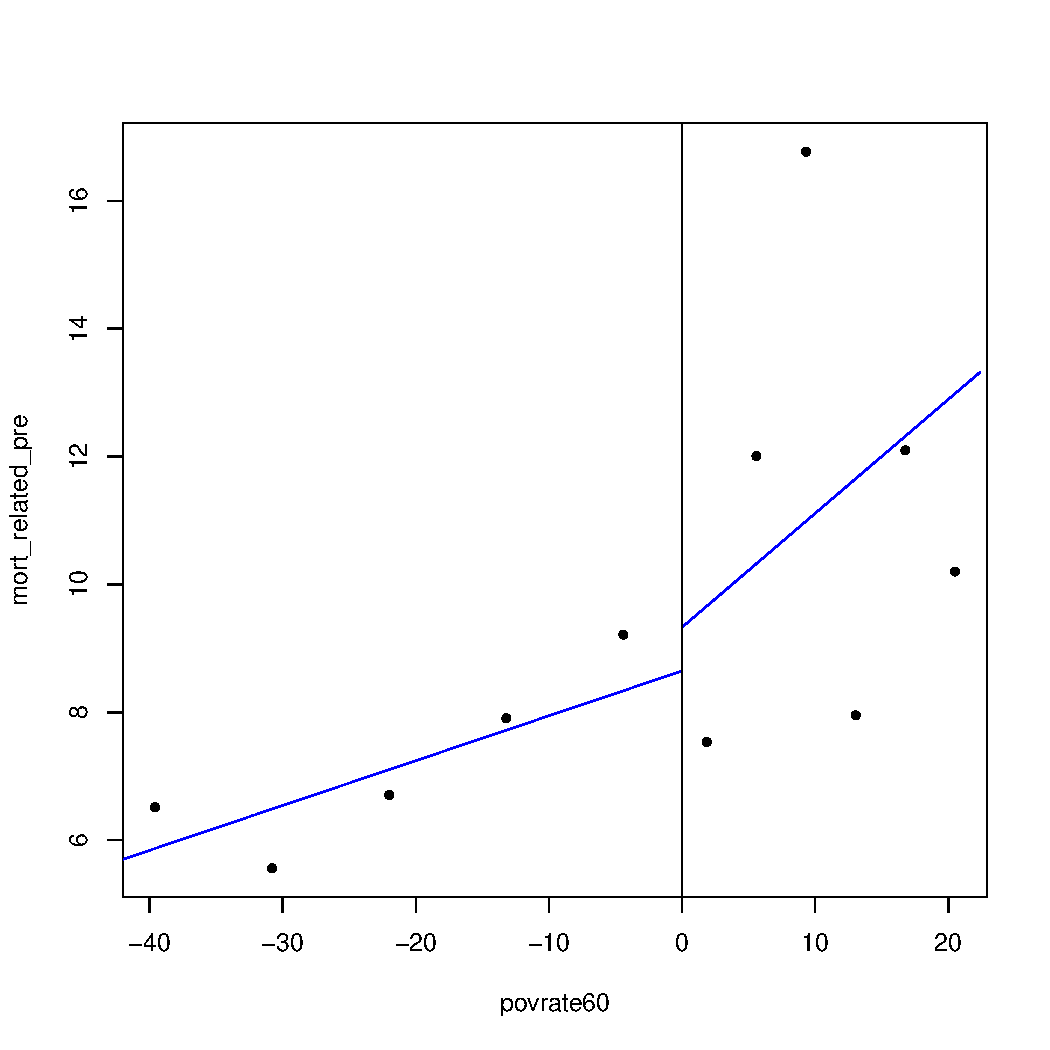
\includegraphics[width=1\textwidth]{q2-1-es.pdf}
        \subcaption{Evenly-spaced, IMSE optimal}
    \end{minipage}\hfill
    \begin{minipage}{0.5\textwidth}
      %  \centering
        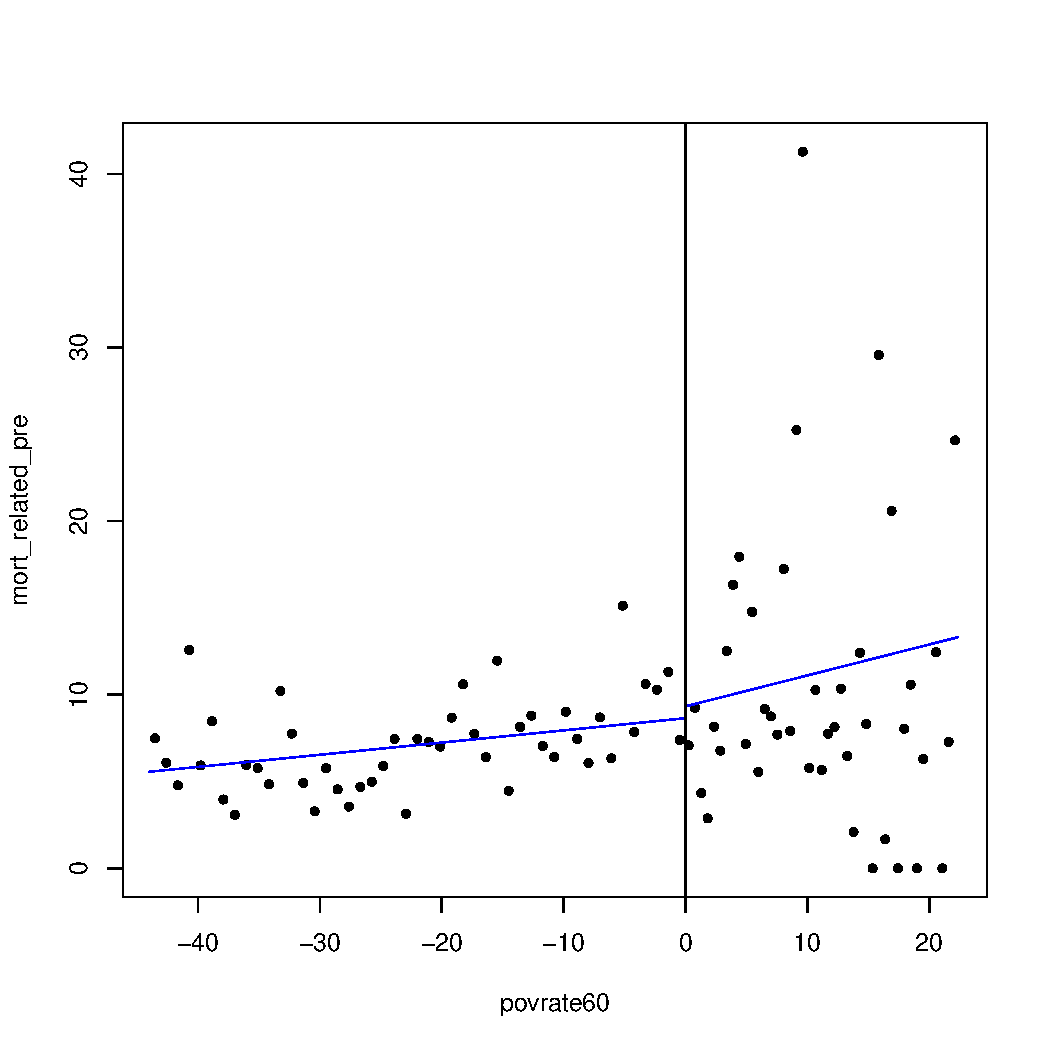
\includegraphics[width=1\textwidth]{q2-1-esmv.pdf}
        \subcaption{Evenly-spaced, variance mimicking}
    \end{minipage}
\centering
\begin{minipage}{0.5\textwidth}
        %\centering
        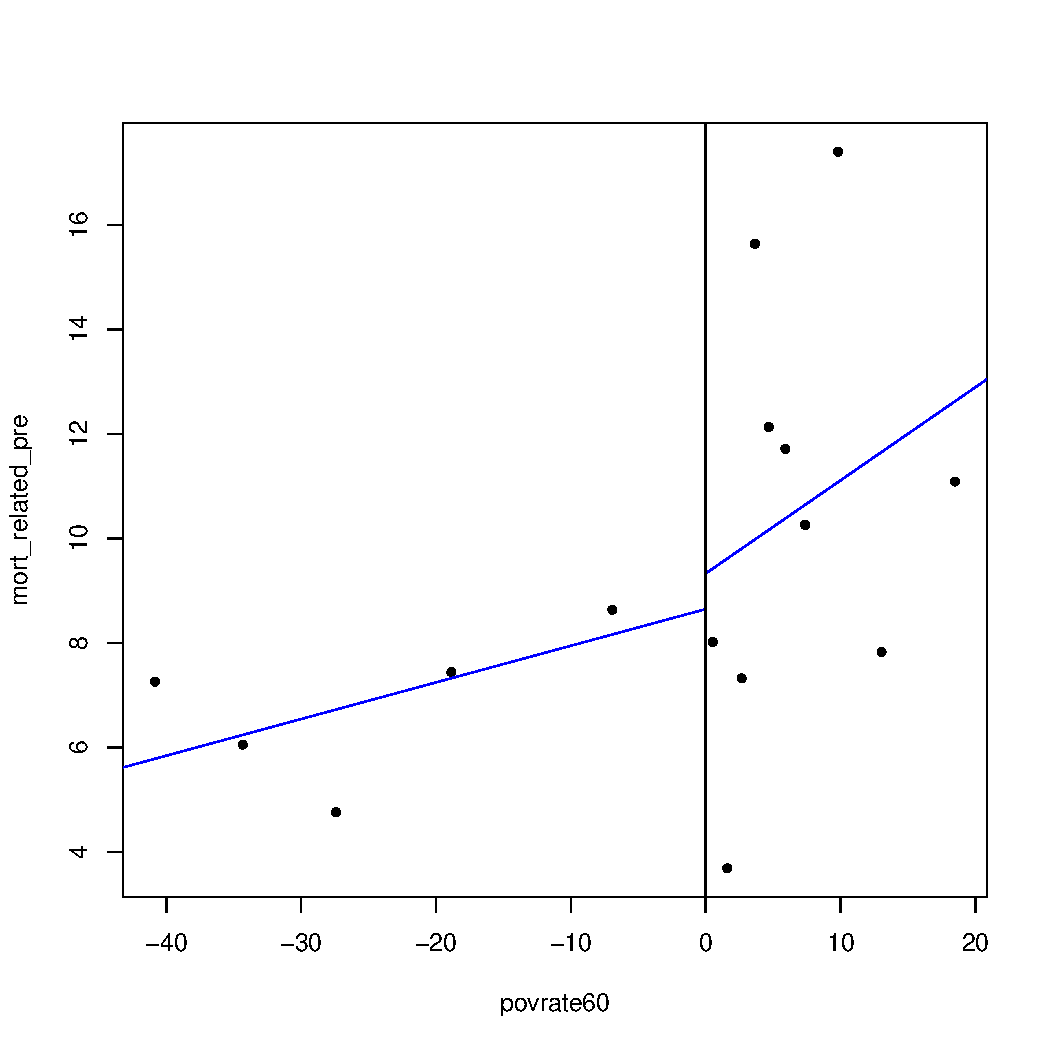
\includegraphics[width=1\textwidth]{q2-1-qs.pdf}
        \subcaption{Quantile-spaced, IMSE optimal}
    \end{minipage}\hfill
    \begin{minipage}{0.5\textwidth}
      %  \centering
        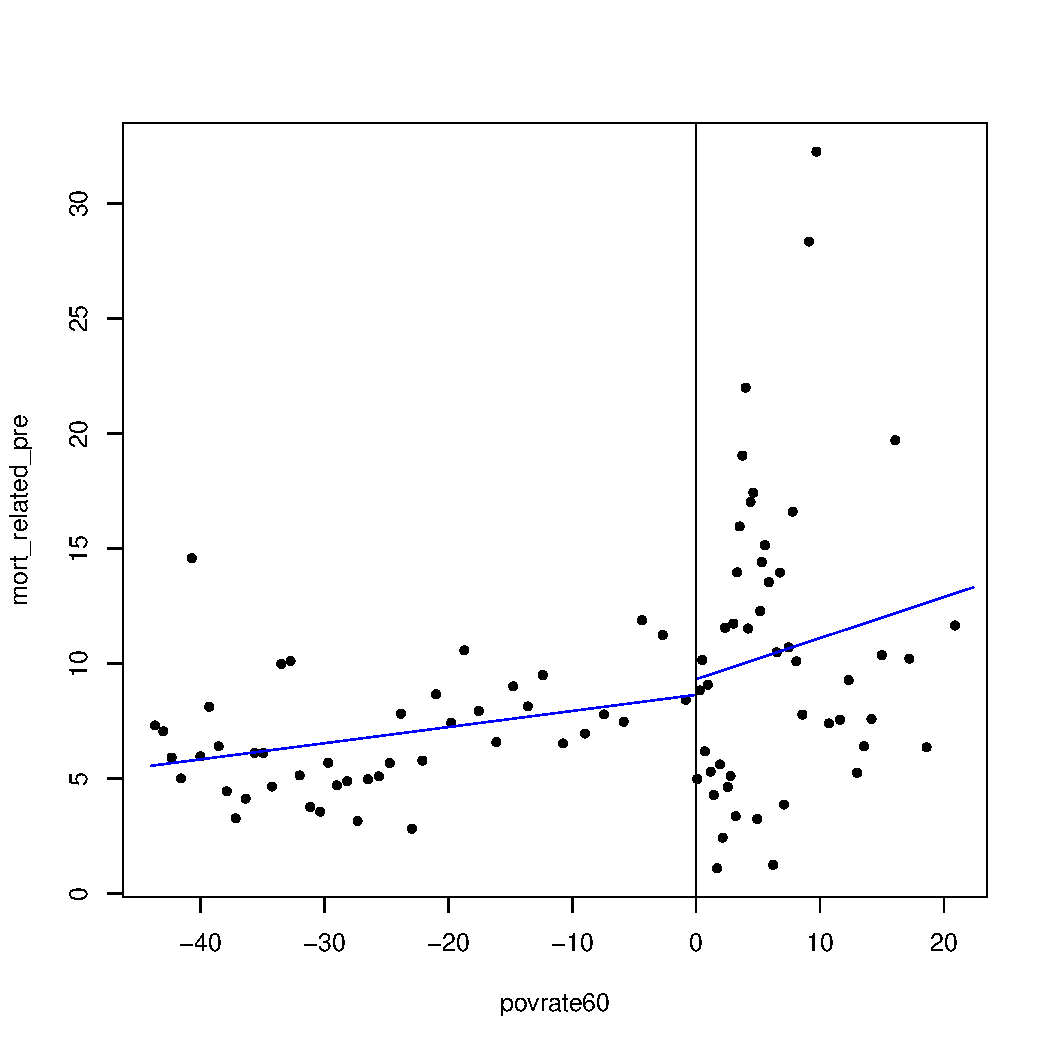
\includegraphics[width=1\textwidth]{q2-1-qsmv.pdf}
        \subcaption{Quantile-spaced, variance mimicking}
    \end{minipage}
\end{figure}

Figure 1 shows the RD plots of \verb|mort_related_pre| using different binning procedures, as required. For each binning method, there is clearly no evidence of a negative discontinuity at the cutoff poverty rate. (In fact, there seems to be a small positive jump in pre-invervention mortality rates at the cutoff.) If there was a negative jump in pre-intervention mortality rates at the cutoff this would potentially falsify the proposed RD design because it would provide strong evidence that the counties assigned to Head Start treatment had systematically lower mortality rates prior to the intervention.\\

We can also conduct formal falsification tests.







\end{document}
